\chapter{Controller Implementation}
\definecolor{ApiLstKeywordColor}{rgb}{0,0,0.4}
\lstset{
  extendedchars=false,
  alsoletter={-},
  basicstyle=\small\fontfamily{txtt}\fontseries{b}\selectfont,
  keywordstyle=\color{ApiLstKeywordColor}\selectfont,
  commentstyle=\color{black!60}\selectfont,
}
\lstdefinestyle{ApiLstStyle}{
  language=java,
  morekeywords={enum, atomic_type},
  breaklines=true,
  breakatwhitespace=true,
  breakautoindent=true,
}

\providecounter{ApiCounter}
\providecommand{\ApiLabel}[1]{\refstepcounter{ApiCounter}\label{#1}}

%%%%%%%%%%%%%%%%%%%%%%%%%%%%%%%%%%%%%%%%%%%%%%%%%%%%%%%%%%%%%%%%%%%%%%%%%%%%%%%%
% API definition
\provideenvironment{Api}{\begin{itemize}}{\end{itemize}}

%%%%%%%%%%%%%%%%%%%%%%%%%%%%%%%%%%%%%%%%%%%%%%%%%%%%%%%%%%%%%%%%%%%%%%%%%%%%%%%%
% API definition code and value
\providecommand{\ApiCode}[1]{\lstinline[style=ApiLstStyle]{#1}}
\providecommand{\ApiValue}[1]{\texttt{#1}}
% \end{verbatim}
% Previous line corrects syntax coloring parser

%%%%%%%%%%%%%%%%%%%%%%%%%%%%%%%%%%%%%%%%%%%%%%%%%%%%%%%%%%%%%%%%%%%%%%%%%%%%%%%%
% API definition item
\providecommand{\ApiItem}[1]{\item #1 %

% Previous empty line is intended to be blank (wraps the text
% to the next line even if the \ApiItem is not followed by empty line)
}

%%%%%%%%%%%%%%%%%%%%%%%%%%%%%%%%%%%%%%%%%%%%%%%%%%%%%%%%%%%%%%%%%%%%%%%%%%%%%%%%
% API command
\provideenvironment{ApiCmd}[2]{{\item \ApiRef{#1} \ApiCode{#2(}}%
\def\ApiCmdTmpFirst{\boolean{true}}%
}{\ApiCode{)}%

% Previous empty line is intended to be blank
}
\provideenvironment{ApiCmdCollection}[3]{{\item \ApiCode{#1<}\ApiRef{#2}\ApiCode{>} \ApiCode{#3(}}%
\def\ApiCmdTmpFirst{\boolean{true}}%
}{\ApiCode{)}%

% Previous empty line is intended to be blank
}
\providecommand{\ApiCmdParam}[2]{%
\ifthenelse{\ApiCmdTmpFirst}{}{, }%
\ApiRef{#1} \ApiCode{#2}%
\def\ApiCmdTmpFirst{\boolean{false}}%
}

%%%%%%%%%%%%%%%%%%%%%%%%%%%%%%%%%%%%%%%%%%%%%%%%%%%%%%%%%%%%%%%%%%%%%%%%%%%%%%%%
% API atomic type
\providecommand{\ApiType}[2]{\ApiLabel{api:#1}\ApiItem{%
  \ifx&#2& \ApiCode{atomic_type #1} \else \ApiCode{atomic_type #1 =\ }\ApiRef{#2} \fi}%
}

%%%%%%%%%%%%%%%%%%%%%%%%%%%%%%%%%%%%%%%%%%%%%%%%%%%%%%%%%%%%%%%%%%%%%%%%%%%%%%%%
% API class
\providecommand{\ApiClass}[2]{\ApiLabel{api:#1}\ApiItem{%
  \ifx&#2& \ApiCode{class #1} \else \ApiCode{class #1 extends\ }\ApiRef{#2} \fi}%
}

%%%%%%%%%%%%%%%%%%%%%%%%%%%%%%%%%%%%%%%%%%%%%%%%%%%%%%%%%%%%%%%%%%%%%%%%%%%%%%%%
% API class attributes
\provideenvironment{ApiClassAttributes}{% Next empty line is intended to be blank

\begin{samepage}\textbf{Attributes:}\begin{compactitem}}{\end{compactitem}\end{samepage}}
\providecommand{\ApiRequired}{{\color{blue!50!black}\textbf{Required}}}
\providecommand{\ApiOptional}{{\color{gray}\textbf{Optional}}}
\providecommand{\ApiOptionalDefault}[1]{{\color{gray}\textbf{Optional}, default: \ApiValue{#1}}}
\providecommand{\ApiReadOnly}{{\color{red!50!black}\textbf{ReadOnly}}}
\providecommand{\ApiClassAttribute}[3]{\ApiItem{\ApiRef{#2} \ApiCode{#1} \hspace{1mm}(\ifx&#3&\ApiReadOnly\else#3\fi)}}
\providecommand{\ApiClassAttributeCollection}[4]{\ApiItem{\ApiCode{#2<}\ApiRef{#3}\ApiCode{>} \ApiCode{#1} \hspace{1mm}(\ifx&#4&\ApiReadOnly\else#4\fi)}}

%%%%%%%%%%%%%%%%%%%%%%%%%%%%%%%%%%%%%%%%%%%%%%%%%%%%%%%%%%%%%%%%%%%%%%%%%%%%%%%%
% API enum
\providecommand{\ApiEnum}[1]{\ApiLabel{api:#1}\ApiItem{\ApiCode{enum #1}}}
\provideenvironment{ApiEnumValues}{% Next empty line is intended to be blank

\begin{samepage}\textbf{Enumeration values:}\begin{compactitem}}{\end{compactitem}\end{samepage}}
\providecommand{\ApiEnumValue}[2]{\ApiItem{{\ApiCode{#1} \ifx&#2& \else \ApiValue{(#2)} \fi}}}

%%%%%%%%%%%%%%%%%%%%%%%%%%%%%%%%%%%%%%%%%%%%%%%%%%%%%%%%%%%%%%%%%%%%%%%%%%%%%%%%
% API example
\providecommand{\ApiExample}{% Next empty line is intended to be blank

\textbf{Example:}
}

%%%%%%%%%%%%%%%%%%%%%%%%%%%%%%%%%%%%%%%%%%%%%%%%%%%%%%%%%%%%%%%%%%%%%%%%%%%%%%%%
% API note
\providecommand{\ApiNote}{% Next empty line is intended to be blank

\textbf{Note:}
}

%%%%%%%%%%%%%%%%%%%%%%%%%%%%%%%%%%%%%%%%%%%%%%%%%%%%%%%%%%%%%%%%%%%%%%%%%%%%%%%%
% API failures
\provideenvironment{ApiFailures}{\begin{compactitem}}{\end{compactitem}}
\providecommand{\ApiFailure}[1]{\ApiItem{\ApiCode{faultCode = #1}}}

%%%%%%%%%%%%%%%%%%%%%%%%%%%%%%%%%%%%%%%%%%%%%%%%%%%%%%%%%%%%%%%%%%%%%%%%%%%%%%%%
% API ref
\providecommand{\ApiRef}[1]{%
\foreach \ApiTmp [count=\ApiTmpIndex] in{#1}{%
%
\ifthenelse{\ApiTmpIndex > 1}{\ApiCode{|}}{}%
%
\def\tmpResult{\boolean{false}}%
\ifthenelse{\equal{\ApiTmp}{String}}{\def\tmpResult{\boolean{true}}}{}%
\ifthenelse{\equal{\ApiTmp}{void}}{\def\tmpResult{\boolean{true}}}{}%
\ifthenelse{\equal{\ApiTmp}{int}}{\def\tmpResult{\boolean{true}}}{}%
\ifthenelse{\equal{\ApiTmp}{boolean}}{\def\tmpResult{\boolean{true}}}{}%
\ifthenelse{\equal{\ApiTmp}{long}}{\def\tmpResult{\boolean{true}}}{}%
\ifthenelse{\equal{\ApiTmp}{float}}{\def\tmpResult{\boolean{true}}}{}%
\ifthenelse{\equal{\ApiTmp}{byte[]}}{\def\tmpResult{\boolean{true}}}{}%
% 
\ifthenelse{\tmpResult}{%
\textbf{\texttt{\ApiTmp}}
}{%
\hyperref[api:\ApiTmp]{\code{\ApiTmp}}%
}%  
}%
}


\lstset{
  classoffset=1,
  morekeywords={
    % Common
    DateTime, ReadablePartial, PeriodicDateTime, Period, Duration, Interval,
    DateTimeSlot, Person,
    % Capabilities
    TerminalCapability, StandaloneTerminalCapability, VirtualRoomsCapability, 
    AliasProviderCapability,
    % Resources
    Alias, Resource, DeviceResource, ManagedMode,
    % Reservation Requests
    ReservationRequest, ReservationRequestSet, EDUCATION, SCIENCE,
    CompartmentSpecification,
    ExternalEndpointSpecification, ExternalEndpointSetSpecification,
    ExistingEndpointSpecification,
    % Reservations
    Reservation, Compartment, Endpoint, VirtualRoom, ConnectionByAddress, 
    ConnectionByAlias,
    % Enums
    H323, SIP, AdobeConnect, E164, URI
  }
}

This chapter describes the implementation for database of \glspl{g:resource} and allocation of \glspl{g:reservation-request} to \glspl{g:reservation} in \gls{g:controller} from the API point of view.

\section{Resource database}

Each \gls{g:controller} contains persistent database of \glspl{g:resource}. New \glspl{g:resource} can be added to the \gls{g:controller}'s database and existing \glspl{g:resource} can be modified or deleted through the \gls{g:controller}'s API. A running \gls{g:controller} holds it's database of \glspl{g:resource} in memory and when it is restarted it reloads the database from a persistent storage. Class diagram for \glspl{g:resource} that are persisted in the database is shown in fig. \ref{fig:cd_api_resources}.

\begin{figure}[ht!]
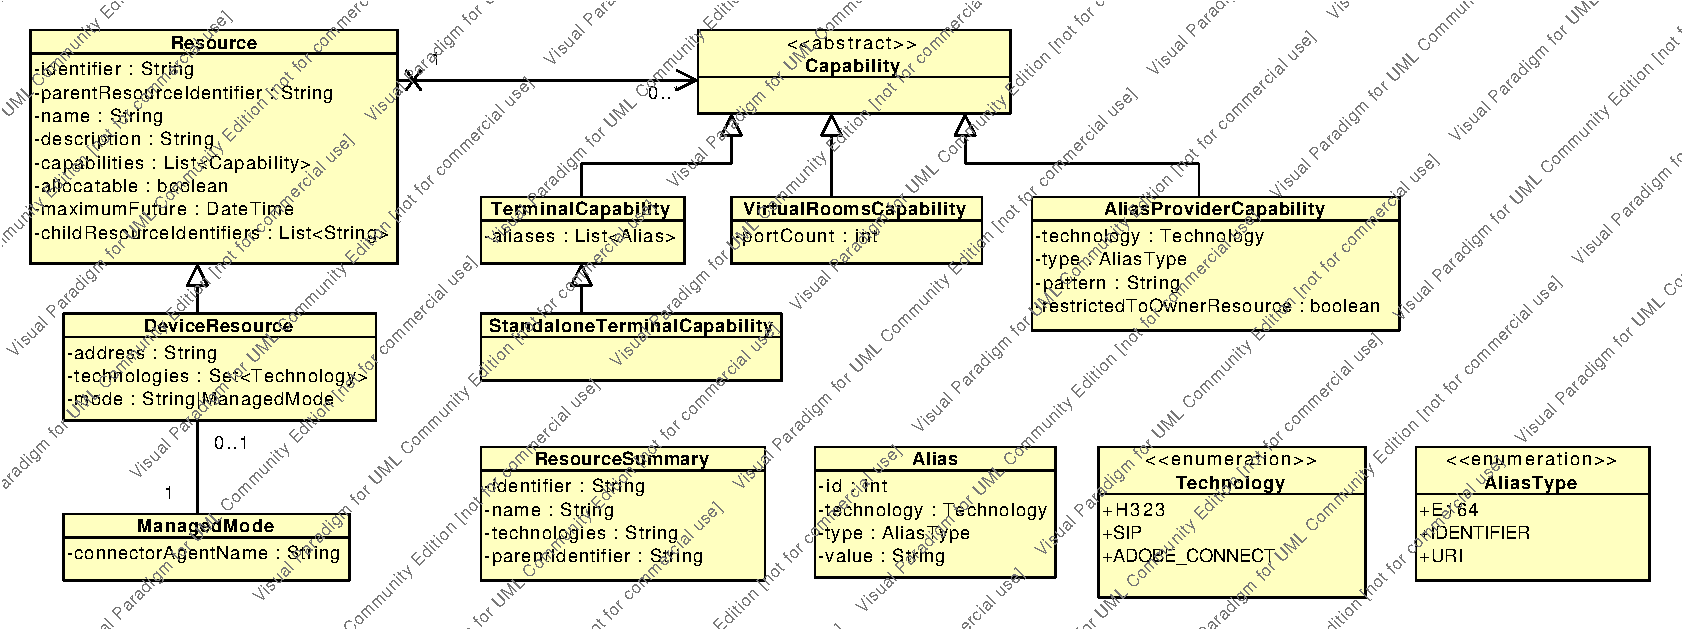
\includegraphics[width=\textwidth]{diagrams/cd_api_resources}
\caption{Class diagram for \gls{g:resource} database in the \gls{g:controller} API}
\label{fig:cd_api_resources}
\end{figure}

A \gls{g:resource} can be created by an instance of \ApiRef{Resource} or \ApiRef{DeviceResource} class. Each \gls{g:resource} is identified by an unique \code{identifier} which is generated by the \gls{g:controller} when the \gls{g:resource} is created in the database. Each resource must have specified if it is \code{allocatable}. If a resource isn't \code{allocatable} a scheduler cannot allocate it to a \gls{g:reservation}. A resource can also have specified \code{maximumFuture} which restrict the \gls{g:controller}'s scheduler to allocate the \gls{g:resource} only to maximum date/time computed as current date/time plus specified \code{maximumFuture}. When a \gls{g:resource} is requested for a \gls{g:reservation} which exceeds the maximum date/time, the scheduler will report an error.

Each resource can have specified zero, one or more \code{capabilities}. Capabality specifies that a \gls{g:resource} provide some feature or service. Some capabilities can be used only for a \ApiRef{DeviceResource} (e.g., \ApiRef{TerminalCapability} or \ApiRef{VirtualRoomsCapability}). Complete description of capabilities can be found in chapter \ref{chapter:controller-api}, but here is a short summary:
\begin{compactitem}
\item \ApiRef{TerminalCapability} tells that a \gls{g:resource-device} can participate in a \gls{g:compartment} (must be connected into a \gls{g:device-virtual-room}, e.g., Adobe Connect client).
\item \ApiRef{StandaloneTerminalCapability} tells that a \gls{g:resource-device} can participate in a \gls{g:compartment}. The compartment may consist only of two \glspl{g:endpoint} without a \gls{g:device-virtual-room} (e.g., H.323 terminal).
\item \ApiRef{VirtualRoomsCapability} tells that a \gls{g:resource-device} can host multiple \glspl{g:device-virtual-room}.
\item \ApiRef{AliasProviderCapability} tells that a \gls{g:resource} can allocate an \gls{g:device-alias} which then can be assigned to a managed \gls{g:endpoint} or a \gls{g:device-virtual-room}.
\end{compactitem}

Here are some examples of resources which can be added to a \gls{g:resource} database in a \gls{g:controller}, e.g., for \ApiValue{cz.cesnet} \gls{g:domain}:

\begin{itemize}

\item Codian MCU which can host multiple H.323 \glspl{g:device-virtual-room} (the limit is 20 ports for all rooms) and which can assign \glspl{g:device-alias} in range \ApiValue{9500872XX} to hosted \glspl{g:device-virtual-room}.

\begin{ObjectCode}{DeviceResource}{mcu}{}
identifier: shongo:cz.cesnet:1,
name: mcu,
description: Codian MCU 4515,
allocatable: true,
maximumFuture: Period(P4M),
technologies: [H323],
capabilities: [
  VirtualRoomsCapability {
    portCount: 20
  },
  AliasProviderCapability {
    technology: H323,
    type: E164,
    pattern: 9500872[dd],
    restrictedToOwnerResource: true 
  }
],
mode: ManagedMode{
  connectorAgentName: codian
}
\end{ObjectCode}

\item Endpoint Tandberg Codec C90 can participate in H.323 \glspl{g:compartment} and it has assigned a H.323 \gls{g:device-alias} \ApiValue{950081038}. 

\begin{ObjectCode}{DeviceResource}{endpoint}{}
identifier: shongo:cz.cesnet:2,
name: endpoint,
description: Tandberg Codec C90,
allocatable: true,
maximumFuture: Period(P4M),
technologies: [H323],
capabilities: [
  StandaloneTerminalCapability {
    aliases: [
      Alias {
        technology: H323,
        type: E164,
        value: 950081038,
      }
    ]
  }
],
mode: ManagedMode{
  connectorAgentName: c90
}
\end{ObjectCode}

\item \Gls{g:resource} representing a physical lecture room.

\begin{ObjectCode}{Resource}{room}{}
identifier: shongo:cz.cesnet:3,
name: room,
description: Lecture room,
allocatable: true,
\end{ObjectCode}


\item Another Tandberg endpoint which is located inside the \code{room} (\ApiValue{shongo:cz.cesnet:3}) and when the endpoint is allocated the room must be also allocated and thus when the room cannot be allocated, the endpoint fails to allocate.

\begin{ObjectCode}{DeviceResource}{anotherEndpoint}{}
identifier: shongo:cz.cesnet:4,
parentIdentifier: ⠶\textcolor{red}{shongo:cz.cesnet:3}⠶,
...
technologies: [H323],
capabilities: [
  StandaloneTerminalCapability {
    ...
  }
],
...
\end{ObjectCode}

\item \Gls{g:resource} that can allocate an \gls{g:device-alias} (H.323 phone number or SIP URI) which then can be assigned to any managed \gls{g:endpoint} or \gls{g:device-virtual-room} in an allocated \gls{g:compartment}.

\begin{ObjectCode}{Resource}{aliasProvider}{}
identifier: shongo:cz.cesnet:5,
name: aliasProvider,
description: Provider for H323 and SIP aliases,
allocatable: true,
maximumFuture: Period(P2Y)
capabilities: [  
  AliasProviderCapability {
    technology: H323,
    type: E164,
    pattern: 9500873[dd],
  }
  AliasProviderCapability {
    technology: SIP,
    type: URI,
    pattern: [ddd]@shongo.cesnet.cz,
  }
]
\end{ObjectCode}

\end{itemize}


\section{Reservation requests}
\label{sec:implementation-reservation-request}

Each controller runs a service component which processes incoming \glspl{g:reservation-request} which can be created by \glspl{g:user} through a \gls{g:controller-client} and the requests are persisted in the \gls{g:controller}'s storage. New \glspl{g:reservation-request} can be created and existing \glspl{g:reservation-request} can be modified or deleted. Class diagram for \glspl{g:reservation-request} is shown in fig. \ref{fig:cd_api_reservation_requests}.

\begin{figure}[ht!]
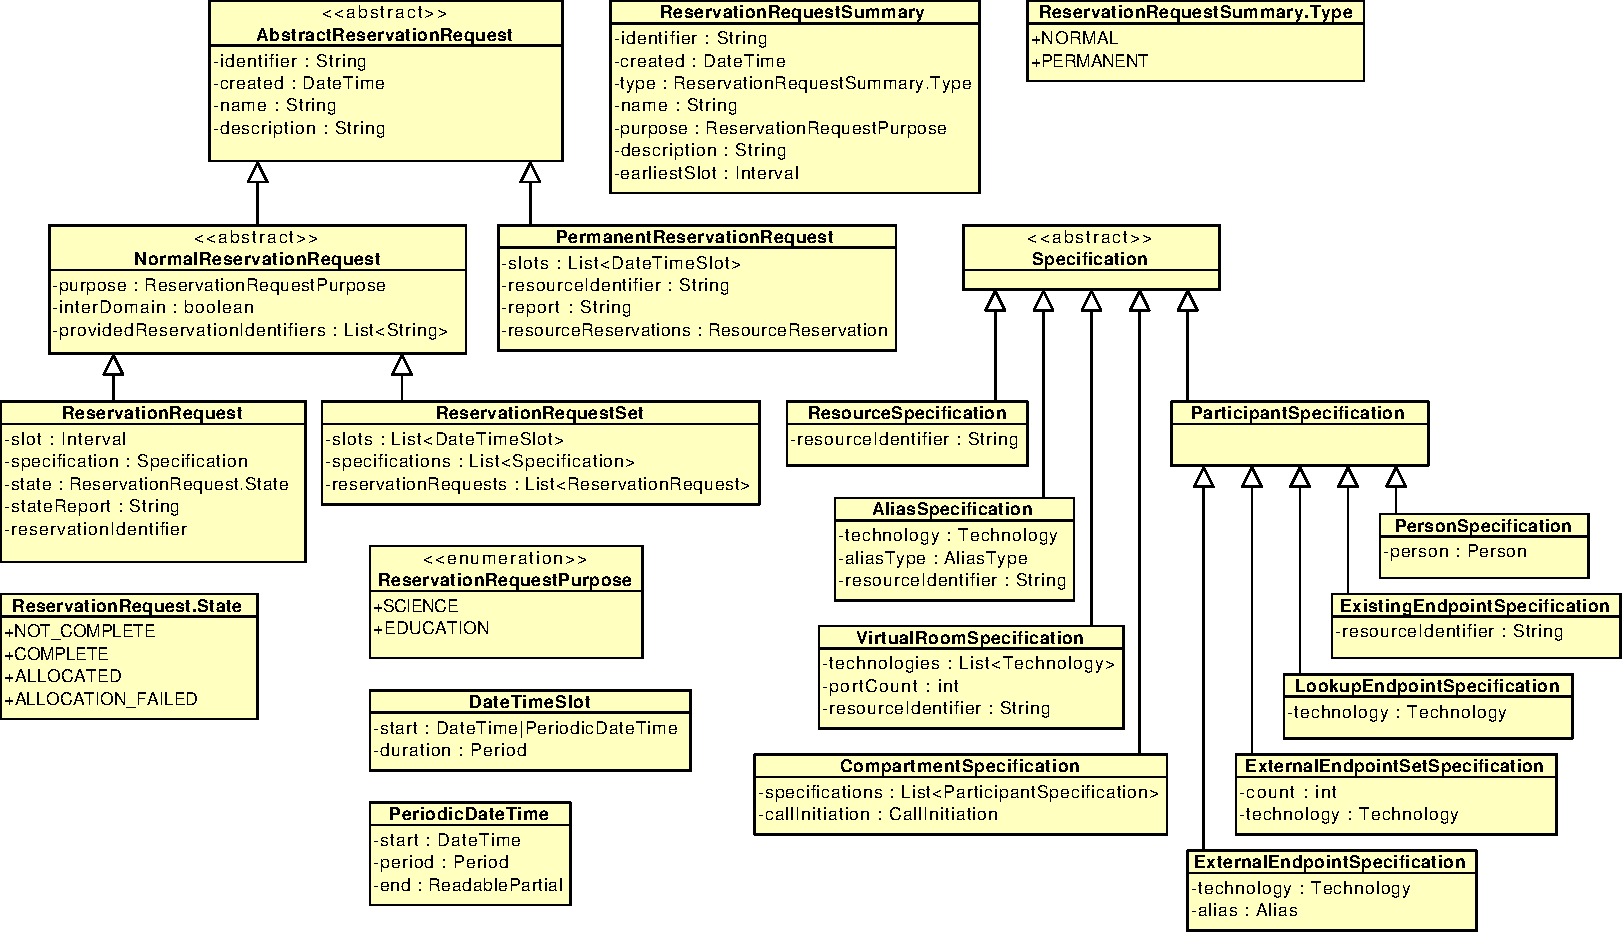
\includegraphics[width=\textwidth]{diagrams/cd_api_reservation_requests}
\caption{Class diagram for \glspl{g:reservation-request} in the \gls{g:controller} API}
\label{fig:cd_api_reservation_requests}
\end{figure}

There are 3 types of \glspl{g:reservation-request}:
\begin{enumerate}
\item \ApiRef{ReservationRequestSet} represents a compound request which can result into multiple \ApiRef{ReservationRequest}s. It must specify one or multiple date/time \code{slots} and one or multiple \code{specifications} for targets which the user wants to get allocated. A single date/time slot can be specified as periodic (e.g., each Tuesday from 14:00 to 16:00 from September to June). 

Multiple date/time slots allows us to specify multiple specific date/times (e.g., today and tomorrow from 13:00 to 15:00) or even multiple periodic date/times (e.g., each Tuesday from 14:00 to 16:00 and Thursday from 16:00 to 18:00 from September to June).

Multiple specifications allows us to request multiple \glspl{g:compartment} or \glspl{g:resource} (e.g., we specify one compartment of H.323 and SIP participants for audio and video and another compartment in web conferencing technology to share content and these two compartments won't be interconnected but will be present at the same date/time slot or slots).

Periodic date/time slots must be enumerated to absolute date/time slots and for each absolute date/time slot and each specification is created one \ApiRef{ReservationRequest} (a Cartesian product of enumerated \code{slots} and \code{specifications}).

\todo{ReservationRequests created for the same date/time slot should be dependent to each other (allocation succeeds for all or none). [not implemented yet]}

\item \ApiRef{ReservationRequest} represents a minimum processable unit for a \gls{g:scheduler} which can be allocated to a \gls{g:reservation}. It must specify exactly one absolute date/time \code{slot} (periodic date/time cannot be used here) and one \code{specification} for a target which should be allocated.

\item \ApiRef{PermanentReservationRequest} represents a special type of request specifying single \gls{g:resource} which should be considered as not-allocatable in specified date/time slots. The request can be created by the \gls{g:resource} owner. It is useful for disabling some date/time slots when the provided resource cannot be used by the \gls{g:scheduler}.
\end{enumerate}
Each \gls{g:reservation-request} is identified by an unique \code{identifier} and each request also has some basic attributes, e.g., date/time when the request was \code{created} or \code{name} of the request).

There are several types of specifications for targets which can be requested for allocation in \glspl{g:reservation-request}:
\begin{enumerate}
\item \ApiRef{ResourceSpecification} allows us to get allocated a specific \gls{g:resource}. Then we can use it in the requested date/time slot for our purposes (e.g., we request a lecture room and we get allocated reservation for the the lecture room and we can do a presentation there).

\item \ApiRef{AliasSpecification} allows us to get allocated an available \gls{g:device-alias}. When we receive an \gls{g:device-alias} \gls{g:reservation} we can use it for our purposes (e.g., assign the \gls{g:device-alias} to our hardware endpoint or installed software client) or we can use it when creating another \gls{g:reservation-request} and pass the \gls{g:device-alias} \gls{g:reservation} to the request. A \gls{g:scheduler} then can use the \gls{g:device-alias} as available resource when it is allocating a \gls{g:reservation} for the \gls{g:reservation-request} (e.g., assign it to any managed \gls{g:endpoint} or created \gls{g:device-virtual-room}). 

\item \ApiRef{ExistingEndpointSpecification} allows us to get allocated a specific \gls{g:endpoint} \gls{g:resource-device}. Then we can use it in the requested date/time slot for our purposes (e.g., we request an H.323 \gls{g:endpoint} in a lecture room and we get allocated reservation for the \gls{g:endpoint} and also for the lecture room, we can go to the lecture room and use the \gls{g:endpoint} to connect to a conference).

\item \ApiRef{LookupEndpointSpecification} allows us to get allocated an \gls{g:endpoint} according to given parameters (e.g., \gls{g:technology} of the \gls{g:endpoint}). The \gls{g:scheduler} will search for an available \gls{g:endpoint} in the \gls{g:resource} database and allocate it for us.

\item \ApiRef{CompartmentSpecification} allows us to get allocated a whole \gls{g:compartment}. We specify one or multiple \code{participants} and the scheduler allocates for us all specified \glspl{g:endpoint} and finds available \glspl{g:device-virtual-room} and \glspl{g:device-alias} which are needed to establish the \gls{g:compartment} and allocates them too. As part of the \ApiRef{CompartmentSpecification} we can also specify \code{callInitiation} -- who should initiate the \gls{g:device-connection} whether a \gls{g:device-virtual-room} or an \gls{g:endpoint} (see \ApiRef{CallInitiation} for more details).

\item \ApiRef{ExternalEndpointSetSpecification} can be specified only inside a \ApiRef{CompartmentSpecification} and it allows us to request a \gls{g:compartment} where should be available ports for external \glspl{g:endpoint} (e.g., user creates a \gls{g:reservation-request} for a \gls{g:compartment} and he specifies that he want 3 external \glspl{g:endpoint} in H.323 and thus the scheduler allocates a \gls{g:reservation} for a single H.323 \gls{g:device-virtual-room} for 3 ports; if the user has also specified one existing \gls{g:endpoint} the scheduler would allocate a H.323 \gls{g:device-virtual-room} for 4 ports).

\item \ApiRef{ExternalEndpointSpecification} can be also specified only inside a \ApiRef{CompartmentSpecification} and it allows us to request a \gls{g:compartment} where should be available port for external \gls{g:endpoint} which can be also \emph{call-out} from a \gls{g:device-virtual-room} (if the specification has \code{alias} specified).

\item \ApiRef{PersonSpecification} can be also specified only inside a \ApiRef{CompartmentSpecification} and it allows us to request a specific person to participate in a \gls{g:compartment}.

\todo{User must be invited to a videoconference (e.g., by email) and he must select an endpoint by which he will connect to the compartment. [not fully implemented yet]}
\end{enumerate}

A \gls{g:reservation-request} (\ApiRef{ReservationRequest}) can be in one of a several states (see fig. \ref{fig:smd_api_reservation_request}):
\begin{enumerate}
\item \code{NOT\_COMPLETE} A \gls{g:reservation-request} is not ready for allocation by a \gls{g:scheduler} (e.g., some person requested by the \ApiRef{PersonSpecification} hasn't confirmed/rejected the invitation or he hasn't selected an endpoint by which he will connect to a \gls{g:compartment}).
\item \code{COMPLETE} A \gls{g:reservation-request} is ready for allocation by a \gls{g:scheduler}, but the \gls{g:scheduler} hasn't allocated it yet.
\item \code{ALLOCATED} A \gls{g:reservation-request} has been successfully allocated by the \gls{g:scheduler} to a \gls{g:reservation}.
\item \code{ALLOCATION\_FAILED} The \gls{g:scheduler} has failed to allocate a \gls{g:reservation-request} to a \gls{g:reservation}.
\end{enumerate}

\begin{figure}[ht!]
\centering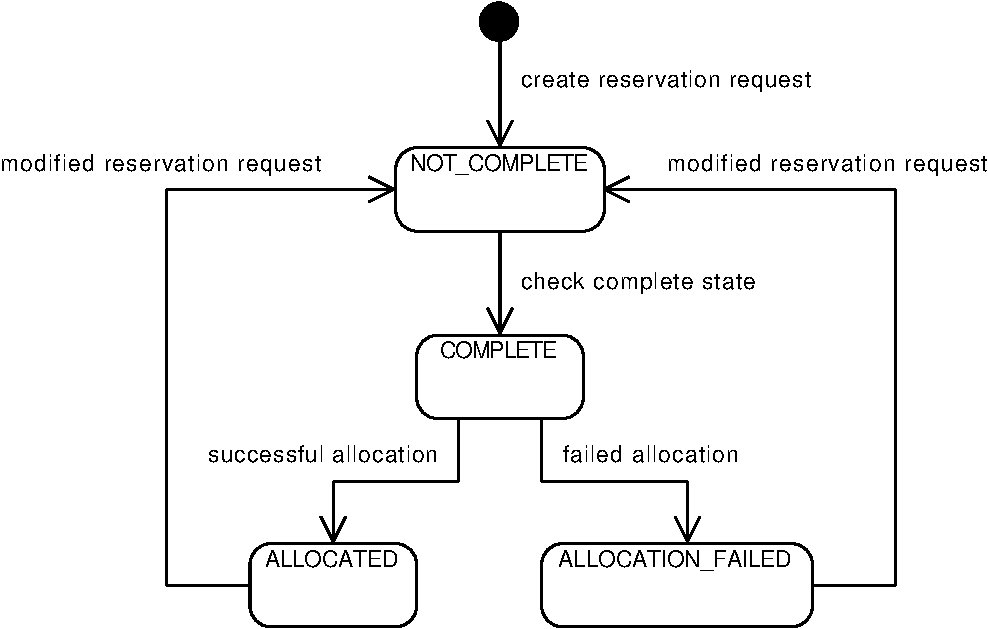
\includegraphics[width=10cm]{diagrams/smd_api_reservation_request}
\caption{State diagram for \gls{g:reservation-request} in the \gls{g:controller} API}
\label{fig:smd_api_reservation_request}
\end{figure}

Only complete \glspl{g:reservation-request} are allocated by the \gls{g:scheduler} to \glspl{g:reservation}.

Here are some examples of \glspl{g:reservation-request}:

\begin{itemize}

\item Permanent \gls{g:reservation-request} which forbids the allocation of Tandberg Codec C90 \gls{g:endpoint} in January 2012.

\label{oc:request1}
\begin{ObjectCode}{PermanentReservationRequest}{request1}{}
identifier: shongo:cz.cesnet:1,
name: Example 1,
slots: [
  DateTimeSlot {
    start: DateTime(2012-01-01T00:00),
    duration: Period(P1M)
  }
],
resourceIdentifier: shongo:cz.cesnet:2 // Tandberg Codec C90
\end{ObjectCode}

\item \Gls{g:reservation-request} for a \gls{g:compartment} taking place on 12.10.2012 from 14:00 to 16:00 in which will participate Tandberg Codec C90 \gls{g:endpoint} from the \gls{g:resource} database (\codeValue{shongo:cz.cesnet:2}) and to the \gls{g:compartment} can also connect any other three H.323 endpoints. Thus for the \gls{g:compartment} must be allocated one H.323 \gls{g:device-virtual-room} with 4 available ports.

\label{oc:request2}
\begin{ObjectCode}{ReservationRequest}{request2}{}
identifier: shongo:cz.cesnet:2,
name: Example 2,
slot: DateTimeSlot {
  start: DateTime(2012-10-12T14:00),
  duration: Period(PT2H)
},
specification: CompartmentSpecification {
  specifications: [
    ExternalEndpointSetSpecification {
      count: 3,
      technology: H323
    },
    ExistingEndpointSpecification { // Tandberg Codec C90
      resourceIdentifier: shongo:cz.cesnet:2
    }
  ]
}
\end{ObjectCode}

\item Set of \glspl{g:reservation-request} from which will be created a \gls{g:reservation-request} for each Wednesday from 14:00 to 16:00, first on 5.9.2012 and last on 26.6.2013. Each created request will be allocated to a \gls{g:compartment} \gls{g:reservation} with a \gls{g:device-virtual-room} for 3 ports in H.323.

\label{oc:request3}
\begin{ObjectCode}{ReservationRequestSet}{request3}{}
identifier: shongo:cz.cesnet:3,
name: Example 3,
slots: [
  DateTimeSlot {
    start: PeriodicDateTime{
      start: DateTime(2012-09-05T14:00),
      period: Period(PT2H),
      end: ReadablePartial(2013-06-31)
    },
    duration: Period(PT2H)
  }
],
specifications: [
  CompartmentSpecification {
    specifications: [
      ExternalEndpointSetSpecification {
        count: 3,
        technology: H323
      }
    ]
  }
]
\end{ObjectCode}

\item \Gls{g:reservation-request} for a H.323 phone number from 1.1.2012 to 31.12.2012.

\label{oc:request4}
\begin{ObjectCode}{ReservationRequest}{request4}{}
identifier: shongo:cz.cesnet:4,
name: Example 4,
slot: DateTimeSlot {
  start: DateTime(2012-01-01T00:00),
  duration: Period(PT1Y)
},
specification: AliasSpecification {
  technology: H323,
  aliasType: E164
}
\end{ObjectCode}

\end{itemize}


\section{Reservations}

\Gls{g:reservation} is an object through which an user receives allocated \glspl{g:resource} which he was requesting by a \gls{g:reservation-request}. Each reservation is identified by an unique \ApiCode{identifier} and the \gls{g:reservation} is allocated for one specific date/time \ApiCode{slot}. Reservation can contain some child \glspl{g:reservation} which has been allocated to satisfy parent allocation needs (e.g., a \gls{g:reservation} for a \gls{g:compartment} may contain child \glspl{g:reservation} for \glspl{g:endpoint}, \glspl{g:device-virtual-room} or \glspl{g:device-alias}, and a \gls{g:reservation} for an \gls{g:endpoint} may contain child \gls{g:reservation} for a lecture room).

\begin{figure}[ht!]
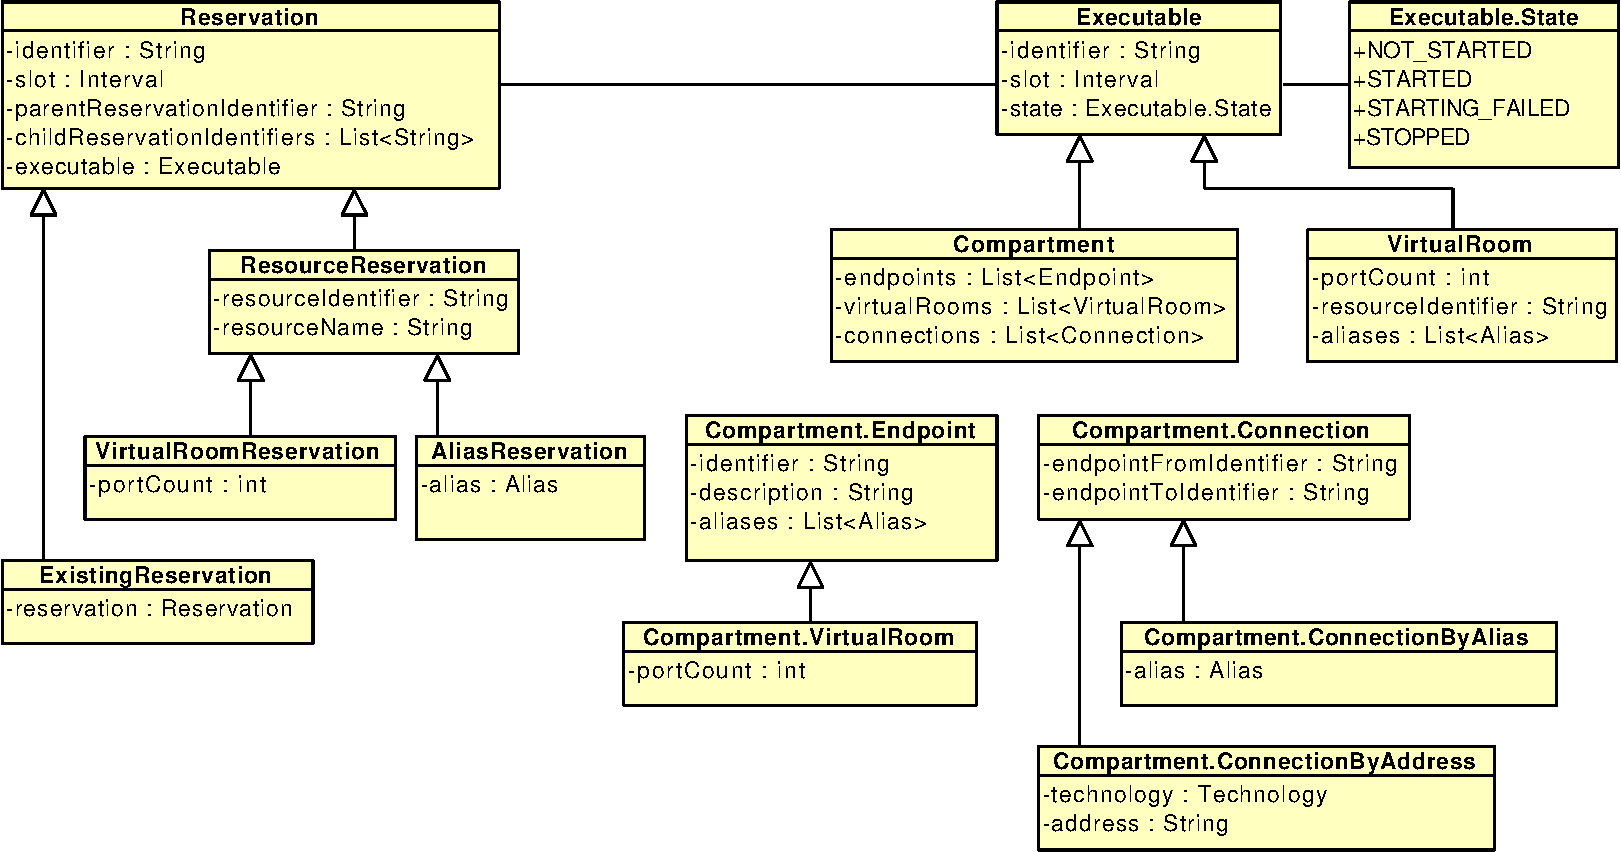
\includegraphics[width=\textwidth]{diagrams/cd_api_reservations}
\caption{Class diagram for \glspl{g:reservation} in the \gls{g:controller} API}
\label{fig:cd_api_reservations}
\end{figure}

There are several types of \glspl{g:reservation}:
\begin{enumerate}
\item \ApiRef{ResourceReservation} represents a \gls{g:reservation} for a \gls{g:resource} from the \gls{g:resource} database (e.g., \gls{g:reservation} for a H.323 \gls{g:endpoint} for a specific date/time slot or a \gls{g:reservation} for a lecture room for a specific date/time slot). For each resource and date/time slot can exist only one reservation (reservation must not collide).

\item \ApiRef{VirtualRoomReservation} represents a special type of \ApiRef{ResourceReservation} for a \gls{g:device-virtual-room} in the \gls{g:resource-device} with a \ApiRef{VirtualRoomsCapability} (e.g., a \gls{g:reservation} for a \gls{g:device-virtual-room} with 5 available ports in H.323 MCU \gls{g:resource}). These \glspl{g:reservation} can collide (multiple \glspl{g:device-virtual-room} can be created at the same time), but must not exceed the maximum number of ports specified in the \ApiRef{VirtualRoomsCapability}.

\item \ApiRef{AliasReservation} represents a special type of \ApiRef{ResourceReservation} for an \ApiCode{alias} from the \gls{g:resource} with an \ApiRef{AliasProviderCapability} (e.g., a \gls{g:reservation} for an \gls{g:device-alias} \ApiValue{950087201} from a \gls{g:resource} which provides \glspl{g:device-alias} with prefix \ApiValue{9500872XX}).

\item \ApiRef{CompartmentReservation} represents a \gls{g:reservation} for a \gls{g:compartment} and it usually contains multiple child \glspl{g:reservation} for \glspl{g:device-virtual-room}, \glspl{g:endpoint} and \glspl{g:device-alias}. It also contains a reference to \ApiCode{compartment} (instance of \ApiRef{Compartment} class) which represents a \gls{g:compartment} plan which is used by an \gls{g:executor} to establish the \gls{g:compartment}.

\item \ApiRef{ExistingReservation} represents a reused \gls{g:reservation} (which was provided in the \gls{g:reservation-request}).
\end{enumerate}

The following two diagrams describes how \ApiRef{ReservationRequest}s and \ApiRef{ReservationRequestSet}s are processed by a \gls{g:controller} and allocated to \ApiRef{Reservation}s (fig. \ref{fig:sd_reservation_request_allocation} and \ref{fig:sd_reservation_request_set_allocation}). Each controller runs these components:
\begin{enumerate}
\item \textbf{Reservation service} accepts new \glspl{g:reservation-request} from users (through \glspl{g:controller-client}) and also new \glspl{g:reservation} from the \gls{g:scheduler} and persist them to \gls{g:controller}'s storage.
\item \textbf{\Gls{g:preprocessor}} uses the service to get not-preprocessed \ApiRef{ReservationRequestSet}s and creates new \ApiRef{ReservationRequest}s from them. \Gls{g:preprocessor} creates only requests which take place in working interval (e.g., one month ahead). It allows an user to create a \ApiRef{ReservationRequestSet} specifying never-ending periodic date/time (e.g., each Thursday from 14:00 to 16:00) and as the weeks goes the \gls{g:preprocessor} will create more and more \ApiRef{ReservationRequest}s.
\item \textbf{\Gls{g:scheduler}} uses the service to get complete \ApiRef{ReservationRequest}s and allocates them to \ApiRef{Reservation}s. The scheduler also allocates only requests in a working interval (e.g., one month ahead).
\end{enumerate}

\begin{figure}[ht!]
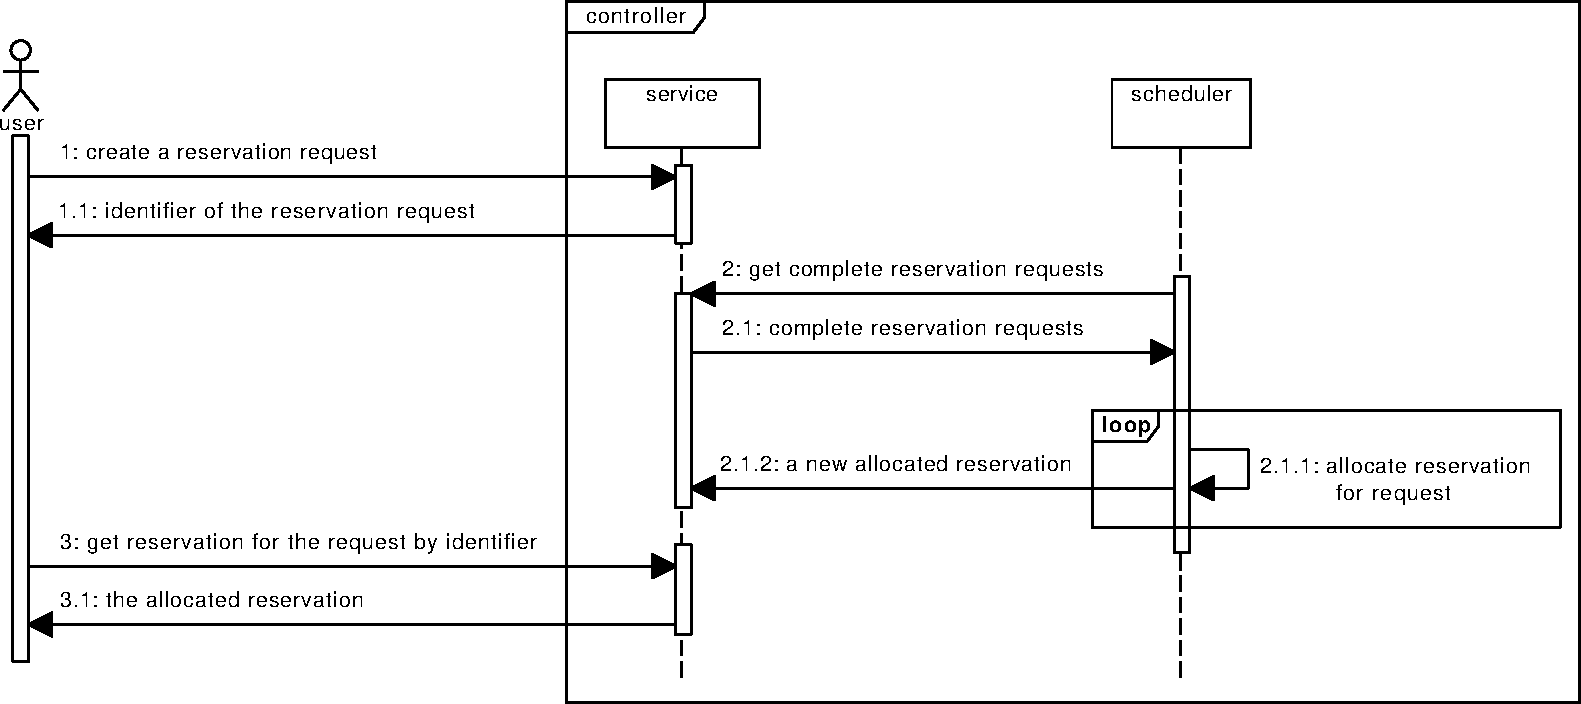
\includegraphics[width=\textwidth]{diagrams/sd_reservation_request_allocation}
\caption{Interaction diagram depicting allocation of \gls{g:reservation} for a single \gls{g:reservation-request}}
\label{fig:sd_reservation_request_allocation}
\end{figure}

\begin{figure}[ht!]
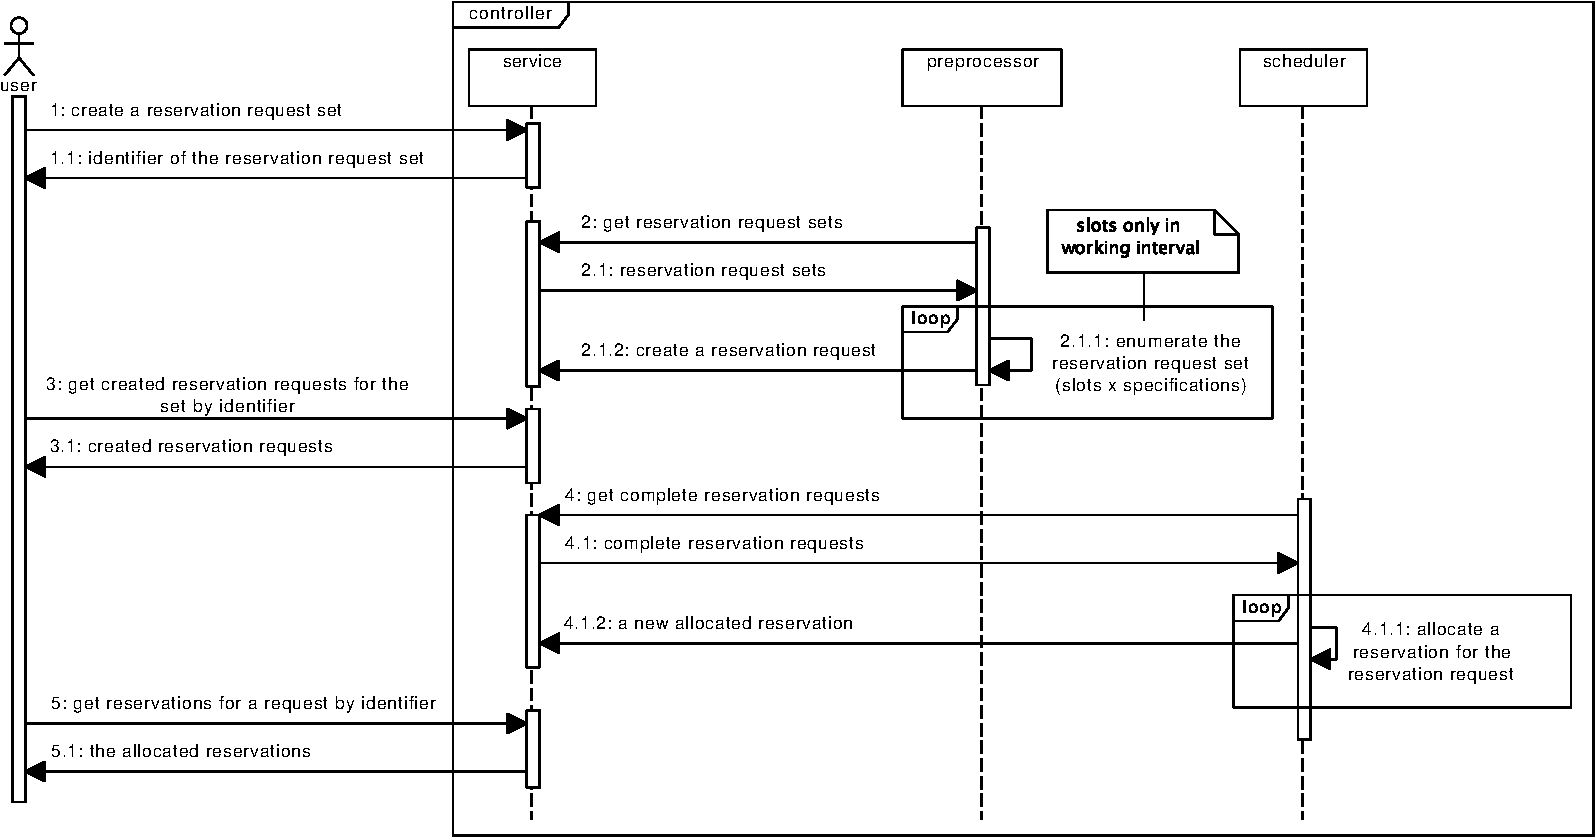
\includegraphics[width=\textwidth]{diagrams/sd_reservation_request_set_allocation}
\caption{Interaction diagram depicting allocation of \glspl{g:reservation} for set of \glspl{g:reservation-request}}
\label{fig:sd_reservation_request_set_allocation}
\end{figure}

\clearpage

Here are some examples of allocated \glspl{g:reservation}:

\begin{itemize}
\item Allocated permanent \gls{g:reservation} for \hyperref[oc:request1]{\codeValue{request1}} (which requested forbidding allocation of Tandberg endpoint) that was described in section \ref{sec:implementation-reservation-request}.
\begin{ObjectCode}{ResourceReservation}{reservation1}{}
identifier: shongo:cz.cesnet:1,
slot: Interval(2012-01-01T00:00/2012-02-01T00:00),
resourceIdentifier: shongo:cz.cesnet:2
\end{ObjectCode}

\item Allocated \gls{g:reservation} for \hyperref[oc:request2]{\codeValue{request2}} (which was requesting compartment for 3 external H.323 ports and existing H.323 \gls{g:endpoint}) that was described in section \ref{sec:implementation-reservation-request}.
\begin{ObjectCode}{CompartmentReservation}{reservation2}{}
identifier: shongo:cz.cesnet:2,
slot: Interval(2012-10-12T14:00/2012-10-12T16:00),
childReservationIdentifiers: [
  shongo:cz.cesnet:3, // Child reservation for Tandberg endpoint 
  shongo:cz.cesnet:4, // Child reservation for virtual room in Codian MCU
  shongo:cz.cesnet:5  // Child reservation for alias for virtual room
],
compartment: Compartment { // Executor compartment plan
  endpoints: [
    Endpoint { // Tandberg Codec C90 endpoint
      identifier: 2,
      description: existing endpoint shongo:cz.cesnet:2,      
    }
  ],
  virtualRooms: [
    VirtualRoom { // Virtual room with 4 available ports in Codian MCU 4515
      identifier: 3,
      portCount: 4,
      description: virtual room in device resource shongo:cz.cesnet:1,      
      aliases: [
        Alias { technology: H323, type: E164, value: 950087201 }
      ]
    }
  ],
  connections: [
    ConnectionByAlias { // Connection from Tandberg endpoint to virtual room
      endpointFromIdentifier: 2, 
      endpointToIdentifier: 3,
      alias: Alias { technology: H323, type: E164, value: 950087201 }
    }
  ]
}
\end{ObjectCode}
\begin{ObjectCode}{ResourceReservation}{reservation3}{Child reservation for Tandberg endpoint}
identifier: shongo:cz.cesnet:3,
slot: Interval(2012-10-12T14:00/2012-10-12T16:00),
parentReservationIdentifier: shongo:cz.cesnet:2,
resourceIdentifier: shongo:cz.cesnet:2
\end{ObjectCode}
\begin{ObjectCode}{VirtualRoomReservation}{reservation4}{Child reservation for virtual room in Codian MCU}
identifier: shongo:cz.cesnet:4,
slot: Interval(2012-10-12T14:00/2012-10-12T16:00),
parentReservationIdentifier: shongo:cz.cesnet:2,
resourceIdentifier: shongo:cz.cesnet:1,
portCount: 4
\end{ObjectCode}
\begin{ObjectCode}{AliasReservation}{reservation5}{Child reservation for alias for virtual room}
identifier: shongo:cz.cesnet:5,
slot: Interval(2012-10-12T14:00/2012-10-12T16:00),
parentReservationIdentifier: shongo:cz.cesnet:2,
resourceIdentifier: shongo:cz.cesnet:1,
alias: Alias { technology: H323, type: E164, value: 950087201 }
\end{ObjectCode}

\item Allocated \gls{g:reservation} for \hyperref[oc:request3]{\codeValue{request3}} on 5.9.2012 (which was requesting compartment for 3 external H.323 ports for multiple date/time slots) that was described in section \ref{sec:implementation-reservation-request}.
\begin{ObjectCode}{CompartmentReservation}{reservation6}{}
identifier: shongo:cz.cesnet:6,
slot: Interval(2012-09-05T14:00/2012-09-05T16:00),
childReservationIdentifiers: [
  shongo:cz.cesnet:7, // Child reservation for virtual room in Codian MCU
  shongo:cz.cesnet:8  // Child reservation for alias for virtual room
],
compartment: Compartment { // Executor compartment plan  
  virtualRooms: [
    VirtualRoom { // Virtual room with 3 available ports in Codian MCU 4515
      identifier: 3,
      portCount: 4,
      description: virtual room in device resource shongo:cz.cesnet:1,      
      aliases: [
        Alias { technology: H323, type: E164, value: 950087201 }
      ]
    }
  ]
}
\end{ObjectCode}
\begin{ObjectCode}{VirtualRoomReservation}{reservation7}{Child reservation for virtual room in Codian MCU}
identifier: shongo:cz.cesnet:7,
slot: Interval(2012-09-05T14:00/2012-09-05T16:00),
parentReservationIdentifier: shongo:cz.cesnet:6,
resourceIdentifier: shongo:cz.cesnet:1,
portCount: 3
\end{ObjectCode}
\begin{ObjectCode}{AliasReservation}{reservation8}{Child reservation for alias for virtual room}
identifier: shongo:cz.cesnet:8,
slot: Interval(2012-09-05T14:00/2012-09-05T16:00),
parentReservationIdentifier: shongo:cz.cesnet:6,
resourceIdentifier: shongo:cz.cesnet:1,
alias: Alias { technology: H323, type: E164, value: 950087201 }
\end{ObjectCode}

\item Allocated \gls{g:reservation} for \hyperref[oc:request4]{\codeValue{request4}} (which was requesting H.323 phone number) that was described in section \ref{sec:implementation-reservation-request}.
\begin{ObjectCode}{AliasReservation}{reservation9}{}
identifier: shongo:cz.cesnet:9,
slot: Interval(2012-01-01T00:00/2013-01-01T00:00),
resourceIdentifier: shongo:cz.cesnet:5, // From aliasProvider resource
alias: Alias { 
  technology: H323, 
  type: E164, 
  value: 950087202 
}
\end{ObjectCode}

\end{itemize}

\todo{Describe that scheduler can in future use inter-controller protocol to allocate resources for reservations}


\section{Authentication \& Authorization}
\label{sec:implementation-authorization}

\subsection{Controller vs. Client}
\Glspl{g:controller-client} communicate with a \gls{g:controller} through XML-RPC \cite{xml-rpc}. When a \gls{g:controller-client} sends a XML-RPC request to a \gls{g:controller} and the request should specify an user identity who sent it (referred to as \emph{secure request}), the request must contain \ApiRef{SecurityToken} as the first parameter. \ApiRef{SecurityToken} equals to OpenID \cite{openid} access token.

Before \gls{g:controller-client} is able to send secure request, it must first obtain an access token for the current user. According to OpenID specification the access token can be obtained from the authorization server as described in fig. \ref{fig:sd_controller_client_authentication}.

\begin{figure}[ht!]
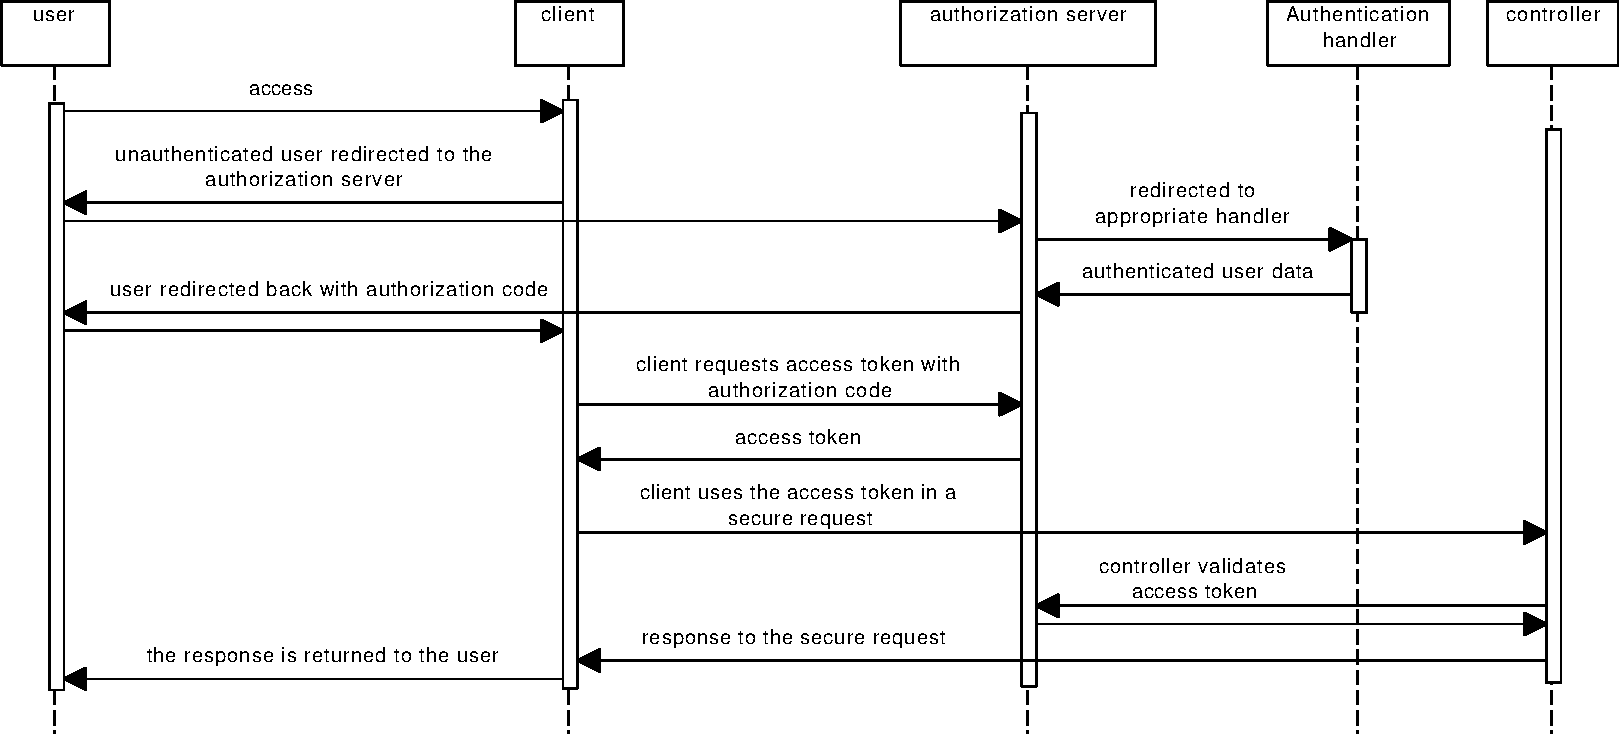
\includegraphics[width=\textwidth]{diagrams/sd_controller_client_authentication}
\caption{Diagram depicting user authentication through \gls{g:controller-client} to \gls{g:controller}}
\label{fig:sd_controller_client_authentication}
\end{figure}

\todo{Describe controller API authorization}

\subsection{Controller vs. Connector}
\todo{Describe connector API authentication}

